\subsection{Physics and Particle Transport}

\paragraph{}
By default, FLUKA transports neutrons down to $1 \times 10^{-5}$ eV or ``thermal energies''. Some other physics processes have to be enabled explicitly using various FLUKA cards. For instance, photo-nuclear events between muons and nuclei are not enabled by default. Figure \ref{fig:physics1} below shows the set of physics cards currently used in the nEXO input file. In all cards with the arguments ``\textcolor{ForestGreen}{Mat:}'' and ``\textcolor{ForestGreen}{to Mat:}'', the respective arguments are ``HYDROGEN'' and ``@LASTMAT''. This simply means that these processes are enabled in all materials from the first to last FLUKA material in the file. Namely, hydrogen has FLUKA material number 1, and the materials used in section \ref{sec:Media} extend to some arbitrary highest integer— @LASTMAT.

\begin{figure}[h]
    \begin{center}
    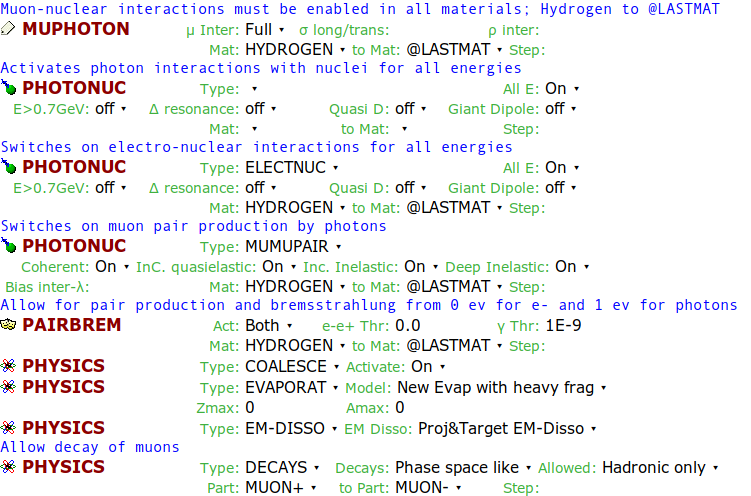
\includegraphics[scale=0.5]{figures/physics.png}
    \caption{The set of physics cards in the nEXO input file}
    \label{fig:physics1}
    \end{center}
\end{figure}

\paragraph{\textcolor{Maroon}{MUPHOTON}}
This is used to enable muon photonuclear interactions and to allow for the production of all secondary hadrons by muons. In this card, the arguments not provided are reserved for code development and not in use.

\paragraph{\textcolor{Maroon}{PHOTONUC}}
These cards are used to activate gamma interactions with nuclei. The first in the series requires only the ``\textcolor{ForestGreen}{All E}'' argument to be ON to enable photonuclear interactions over all energies in FLUKA. The second two \textcolor{Maroon}{PHOTONUC} cards are used to activate electronuclear interactions and muon-muon pair production respectively.

\paragraph{\textcolor{Maroon}{PAIRBREM}}
This card controls simulation of pair production and bremsstrahlung by high-energy muons, charged hadrons and light ions (up to alpha's). Here, both bremsstrahlung and pair production are activated with the electron energy threshold set to 0 which corresponds to the lowest FLUKA limits, and the $\gamma$ threshold set to 1 eV.